% Russian language
\documentclass{article}
\usepackage[utf8]{inputenc}
\usepackage[russian]{babel}

% Math symbols
\usepackage{amssymb}
\usepackage{amsmath}

% Images inplace
\usepackage{float}
\usepackage{graphicx}
% Code blocks
\DeclareFixedFont{\ttb}{T1}{txtt}{bx}{n}{8} % for bold
\DeclareFixedFont{\ttm}{T1}{txtt}{m}{n}{8}  % for normal
\usepackage{color}
\definecolor{deepblue}{rgb}{0,0,0.5}
\definecolor{deepred}{rgb}{0.6,0,0}
\definecolor{deepgreen}{rgb}{0,0.5,0}
\usepackage{listings}
\newcommand\pythonstyle{\lstset{
language=Python,
basicstyle=\ttm,
morekeywords={self},              % Add keywords here
keywordstyle=\ttb\color{deepblue},
emph={MyClass,__init__},          % Custom highlighting
emphstyle=\ttb\color{deepred},    % Custom highlighting style
stringstyle=\color{deepgreen},
frame=tb,                         % Any extra options here
showstringspaces=false
}}
\lstnewenvironment{python}[1][]
{
\pythonstyle
\lstset{#1}
}
{}
\newcommand\pythonexternal[2][]{{
\pythonstyle
\lstinputlisting[#1]{#2}}}
\newcommand\pythoninline[1]{{\pythonstyle\lstinline!#1!}}
% Code blocks

\makeatletter
\renewcommand*\env@matrix[1][*\c@MaxMatrixCols c]{%
  \hskip -\arraycolsep
  \let\@ifnextchar\new@ifnextchar
  \array{#1}}
\makeatother

\title{Лабораторная работа №1}
\author{Ларин Егор. 4 группа 3 курс}

\begin{document}
\maketitle
\section*{Теория}
\subsection*{Задача}
\begin{equation*}
    u' = \frac{u \ln u}{x}, u(1) = e, x \in \left[0, 1\right].
\end{equation*}

Точное решение данного уравнения $u(x) = e^x$.
Для нахождения численного решения введем сетку узлов $ \omega_h = \{x_i = 1 + i
* h : i = \overline{0, N}, N = \frac{(b-a)}{N} \} $ 

\subsection*{Неявный метод трапеций}
\[
    y_{i+1}^0 = y_i
\]
\[
    y_{i+1}^{k+1} = y_{i+1}^k - \frac{y^k_{i+1} - y_i - \frac{1}{2} h (f(x_i,
    y_i), f(x_{i+1}, y^k_{i+1})) }{1- \frac{1}{2} h f_u(x_{i+1}, y^k_{i+1})}
\]
Условие остановки итерационного процесса Ньютона:
\[
    \left|y_i^k - y_i^{k+1} \right| < \varepsilon = 10^{-6}
\]


\subsection*{Явный метод Рунге-Кутта 4-го порядка}
\[
    q = 3, y_{i+1} = y_i + \frac{1}{6}h(\varphi_0 + 2 \varphi_1 + 2\varphi_2 + \varphi_3)
\]
\[
    \begin{cases}
       \varphi_0 = f(x_i, y_i) \\
       \varphi_1 = f(x_i + \frac{1}{2}h, y_i + \frac{1}{2} h \varphi_0) \\
       \varphi_2 = f(x_i + \frac{1}{2}h, y_i + \frac{1}{2} h \varphi_1) \\
       \varphi_3 = f(x_i, y_i + h \varphi_2)
    \end{cases}
\]
\subsection*{Явный метод средних прямоугольников}
\[
    y_{i+1} = y_i + h f(x_i + \frac{h}{2}, y_i + \frac{h}{2}f(x_i, y_i)), y_0 = u(1)
\]

\section*{Листинг кода}
\begin{python}
from math import ceil, exp, log
from matplotlib import pyplot as plt

a = 1.
b = 2.
initial = exp(a)
f = lambda x, y: y * log(y) / x
u = lambda x: exp(x)
dudu = lambda x, y: (log(y) + 1) / x
eps = 0.000001

def runge(h, ass, alpha, beta):
    q = len(ass)
    n = ceil((b - a) / h)
    ys = [initial]
    xs = [a + i * h for i in range(n)]
    for i in range(n-1):
        integral = 0.
        y = ys[-1]
        phi = [f(xs[i], y)]
        for k in range(q):
            if k != 0:
                phi.append(f(xs[i] + h * alpha[k-1], y + h * sum([beta[k-1][j] * phi[k-1] for j in range(k)])))
            integral += ass[k] * phi[k]
        ys.append(y + h * integral)
    norm = max([abs(y - u(x)) for (x, y) in zip(xs, ys)])
    plt.plot(xs, ys, "ro", xs, [u(x) for x in xs], "b")
    plt.legend(["$y(x)$", "$e^x$"])
    plt.title(f"$q = {q}$, $h = {h}$, norm = ${norm}$")
    plt.show()
    print(f"q = {q}, h = {h}, norm = {norm}")

def euler(h):
    n = ceil((b - a) / h)
    ys = [initial]
    xs = [a + i * h for i in range(n)]
    for i in range(n-1): 
        last = ys[-1]
        while True:
            current = last - (last - ys[-1] - 0.5 * h * (f(xs[i], ys[-1]) + f(xs[i+1], last)))/(1 - 0.5 * h * dudu(xs[i+1], last))
            if abs(last - current) < eps:
                ys.append(current)
                break
            last = current
    norm = max([abs(y - u(x)) for (x, y) in zip(xs, ys)])
    plt.plot(xs, ys, "ro", xs, [u(x) for x in xs], "b")
    plt.legend(["$y(x)$", "$e^x$"])
    plt.title(f"Euler $h = {h}$, norm = ${norm}$")
    plt.show()
    print(f"Euler h = {h}, norm = {norm}")
\end{python}
\section*{Графики}
\begin{figure}[H]
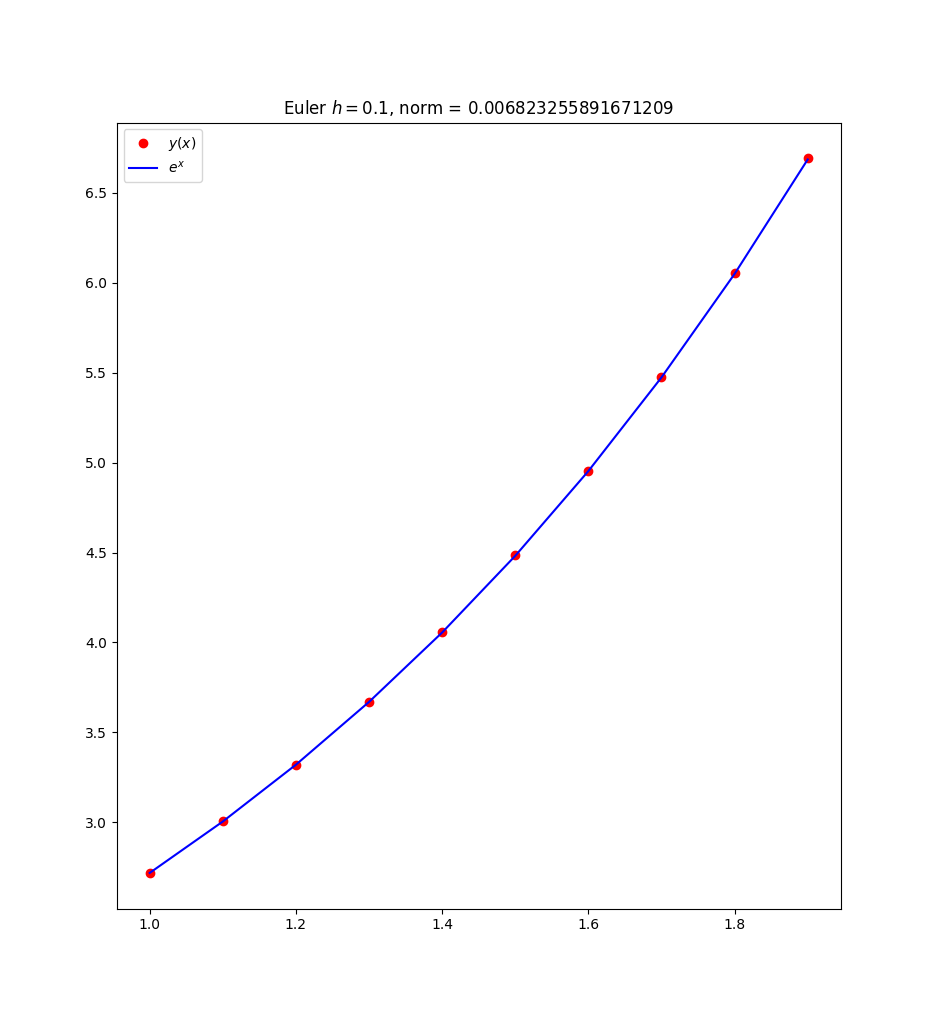
\includegraphics[width=0.5\textwidth]{Figure_1.png}
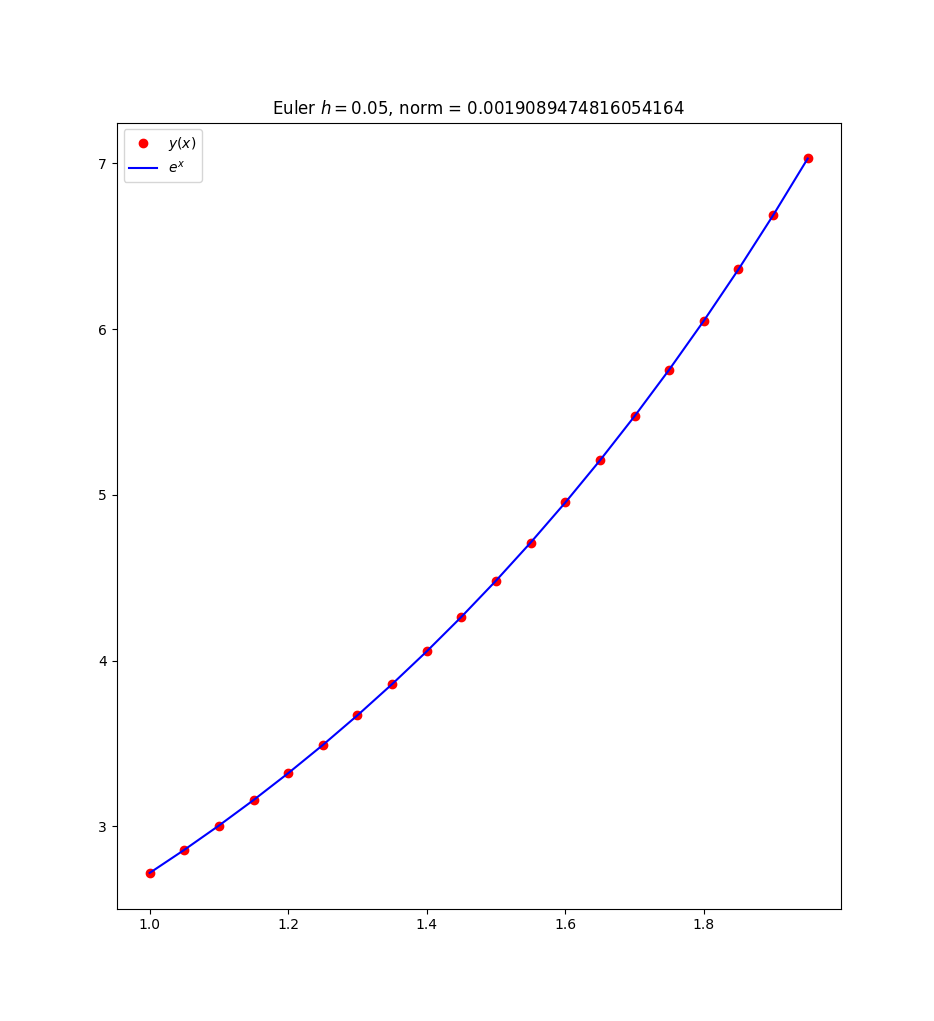
\includegraphics[width=0.5\textwidth]{Figure_2.png}
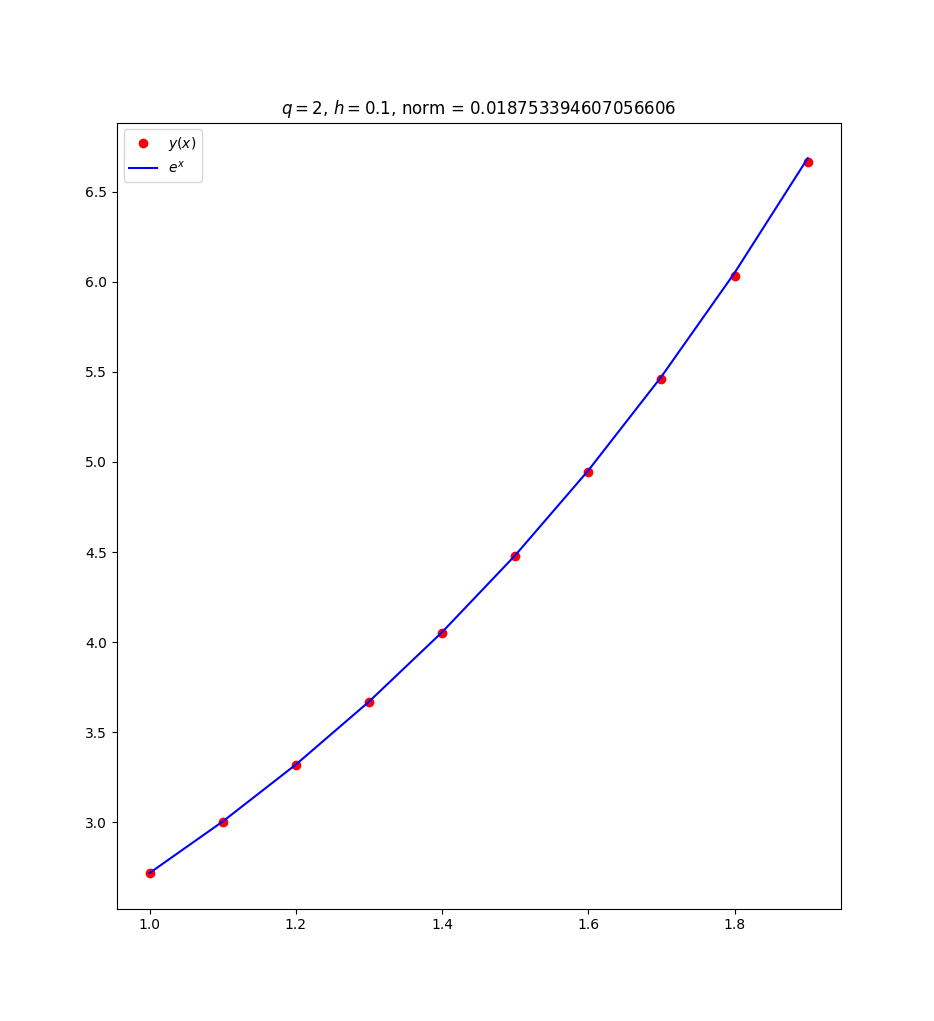
\includegraphics[width=0.5\textwidth]{Figure_3.png}
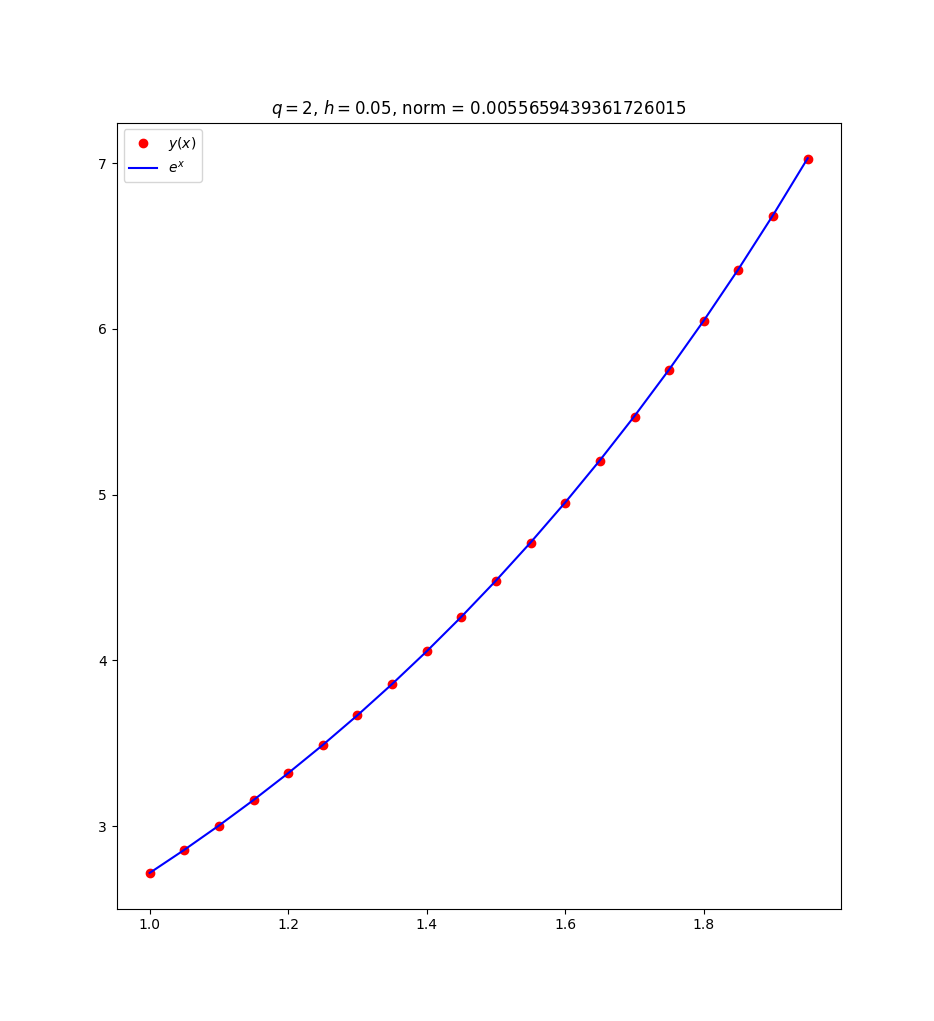
\includegraphics[width=0.5\textwidth]{Figure_4.png}
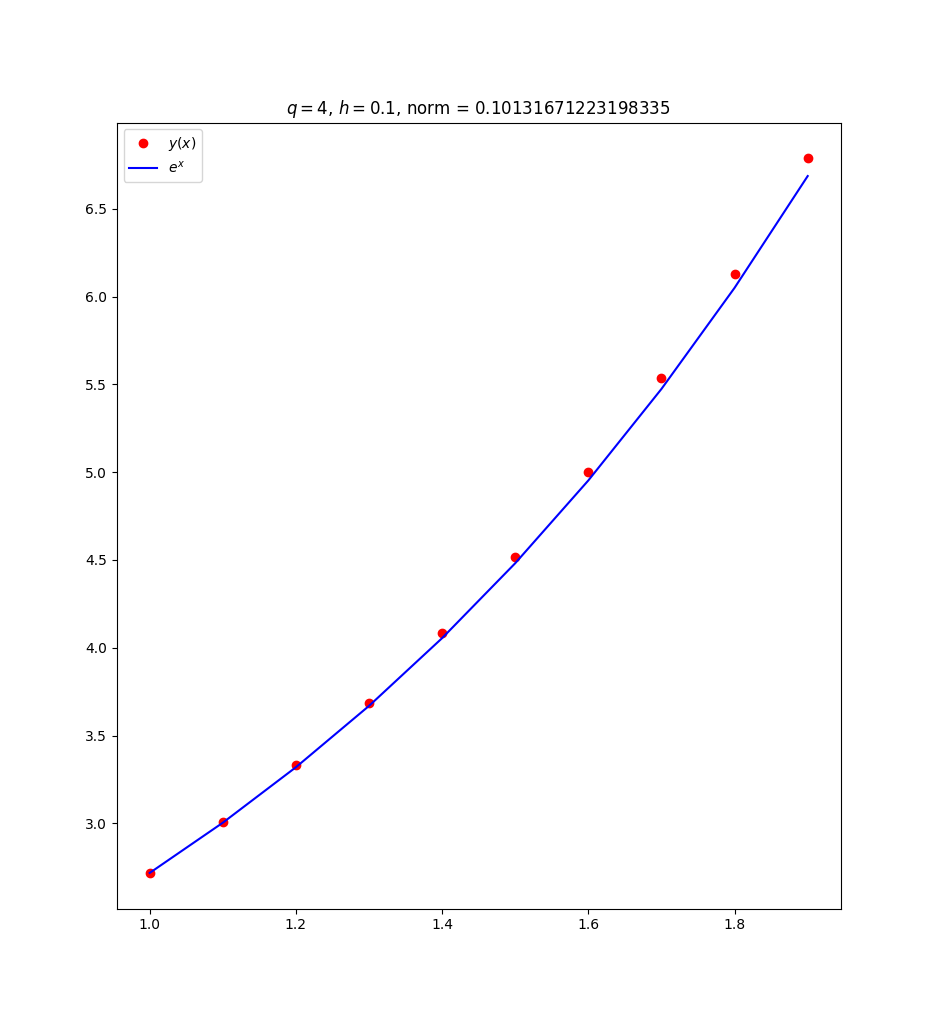
\includegraphics[width=0.5\textwidth]{Figure_5.png}
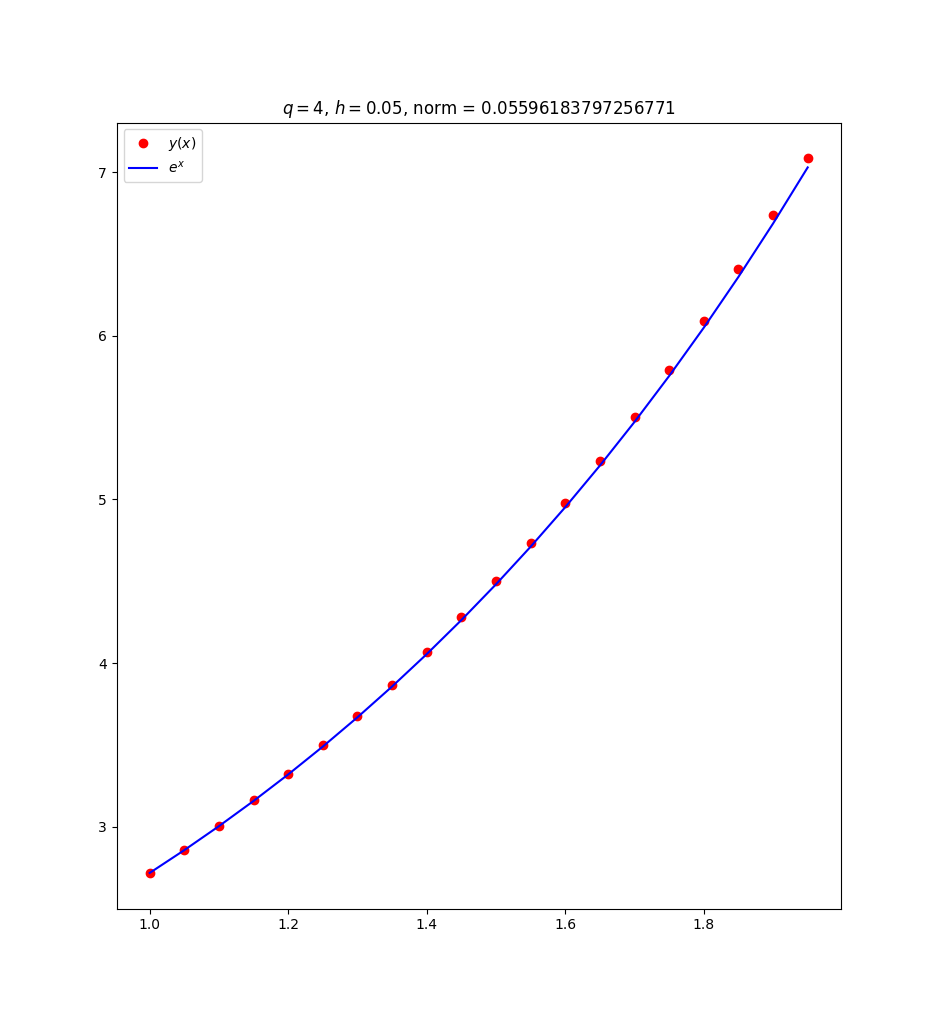
\includegraphics[width=0.5\textwidth]{Figure_6.png}
\end{figure}

\section*{Результаты вычислительного эксперимента}
\begin{tabular}[H]{|l|l|l|}
  \hline
  Метод & $h$ & Погрешность \\
  \hline
  НМТ &   0.1         &    0.006823255891671209 \\
  НМТ &   0.05        & 0.0019089474816054164    \\
  ЯСП &   0.1         &  0.018753394607056606   \\
  ЯСП &   0.05        &   0.0055659439361726015  \\
  $   q=4 $    & 0.1  & $3.70279931267703 \cdot 10^{-5}$  \\
  $   q=4 $    & 0.05 &  $2.7515251455056955 \cdot 10^{-6}$ \\
  \hline
\end{tabular} 
\section*{Выводы}
Вычислительный эксперимент показал, что более высокий порядок аппроксимации
метода не гарантирует меньшую погрешность полученного решения и что при
достаточно малом количестве вычислений оба метода дают относительно небольшую
погрешность.
\end{document}
